\documentclass[]{elsarticle} %review=doublespace preprint=single 5p=2 column
%%% Begin My package additions %%%%%%%%%%%%%%%%%%%
\usepackage[hyphens]{url}
\usepackage{lineno} % add
\providecommand{\tightlist}{%
  \setlength{\itemsep}{0pt}\setlength{\parskip}{0pt}}

\bibliographystyle{elsarticle-harv}
\biboptions{sort&compress} % For natbib
\usepackage{graphicx}
\usepackage{booktabs} % book-quality tables
%% Redefines the elsarticle footer
%\makeatletter
%\def\ps@pprintTitle{%
% \let\@oddhead\@empty
% \let\@evenhead\@empty
% \def\@oddfoot{\it \hfill\today}%
% \let\@evenfoot\@oddfoot}
%\makeatother

% A modified page layout
\textwidth 6.75in
\oddsidemargin -0.15in
\evensidemargin -0.15in
\textheight 9in
\topmargin -0.5in
%%%%%%%%%%%%%%%% end my additions to header

\usepackage[T1]{fontenc}
\usepackage{lmodern}
\usepackage{amssymb,amsmath}
\usepackage{ifxetex,ifluatex}
\usepackage{fixltx2e} % provides \textsubscript
% use upquote if available, for straight quotes in verbatim environments
\IfFileExists{upquote.sty}{\usepackage{upquote}}{}
\ifnum 0\ifxetex 1\fi\ifluatex 1\fi=0 % if pdftex
  \usepackage[utf8]{inputenc}
\else % if luatex or xelatex
  \usepackage{fontspec}
  \ifxetex
    \usepackage{xltxtra,xunicode}
  \fi
  \defaultfontfeatures{Mapping=tex-text,Scale=MatchLowercase}
  \newcommand{\euro}{€}
\fi
% use microtype if available
\IfFileExists{microtype.sty}{\usepackage{microtype}}{}
\usepackage{graphicx}
% We will generate all images so they have a width \maxwidth. This means
% that they will get their normal width if they fit onto the page, but
% are scaled down if they would overflow the margins.
\makeatletter
\def\maxwidth{\ifdim\Gin@nat@width>\linewidth\linewidth
\else\Gin@nat@width\fi}
\makeatother
\let\Oldincludegraphics\includegraphics
\renewcommand{\includegraphics}[1]{\Oldincludegraphics[width=\maxwidth]{#1}}
\ifxetex
  \usepackage[setpagesize=false, % page size defined by xetex
              unicode=false, % unicode breaks when used with xetex
              xetex]{hyperref}
\else
  \usepackage[unicode=true]{hyperref}
\fi
\hypersetup{breaklinks=true,
            bookmarks=true,
            pdfauthor={},
            pdftitle={Food-web complexity flattens the fitness landscape of an insect herbivore},
            colorlinks=true,
            urlcolor=blue,
            linkcolor=magenta,
            pdfborder={0 0 0}}
\urlstyle{same}  % don't use monospace font for urls
\setlength{\parindent}{0pt}
\setlength{\parskip}{6pt plus 2pt minus 1pt}
\setlength{\emergencystretch}{3em}  % prevent overfull lines
\setcounter{secnumdepth}{0}
% Pandoc toggle for numbering sections (defaults to be off)
\setcounter{secnumdepth}{0}
% Pandoc header


\usepackage[nomarkers]{endfloat}

\begin{document}
\begin{frontmatter}

  \title{Food-web complexity flattens the fitness landscape of an insect
herbivore}
    \author[Department of Evolutionary Biology and Environmental Studies, University
of Zurich, Zurich, Switzerland]{Matthew A. Barbour\corref{c1}}
   \ead{matthew.barbour@ieu.uzh.ch} 
   \cortext[c1]{Corresponding Author}
    \author[Another University]{Jordi Bascompte}
   \ead{jordi.bascompte@ieu.uzh.ch} 
  
      \address[Some Institute of Technology]{Department, Street, City, State, Zip}
    \address[Another University]{Department, Street, City, State, Zip}
  
  \begin{abstract}
  true
  \end{abstract}
  
 \end{frontmatter}

\emph{Text based on elsarticle sample manuscript, see
\url{http://www.elsevier.com/author-schemas/latex-instructions\#elsarticle}}

\begin{quote}
\emph{There is a much more insidious kind of extinction: the extinction
of ecological interactions.} \emph{(Janzen, D.H. 1974. The deflowering
of Central America. Natural History. 83:48--53).}
\end{quote}

\section{Introduction}\label{introduction}

Biological diversity -- from genes, to phenotypes, to species -- has and
continues to be shaped by the interplay between ecological and
evolutionary processes. Much of this biological diversity has been
molded by natural selection arising from species interactions, such as
resource competition (Schluter (2000)), mutualisms (Jordano (1987)), and
predation (Abrams (2000)). While there is clear evidence that pairwise
interactions can drive evolution, we also know that most species
interact with multiple species in an ecological community. Understanding
how evolutionary dynamics unfold in a community context is challenging
and eminently theoretical (Mcpeek (2017), Mazancourt, Johnson, and
Barraclough (2008), Guimarães et al. (2017), Nuismer, Jordano, and
Bascompte (2013)). Given the rapid loss of species diversity we are
experiencing throughout the world (cite), we are in urgent need of work
that makes and tests predictions for how the loss of species will affect
the evolutionary process in natural communities.

Predicting the evolutionary consequences of species loss first requires
an understanding of the concommitant change in the species-interaction
networks. Knowing the interaction network is crucial because the loss of
biodiversity, in and of itself, will not alter evolution -- it is the
associated loss of ecological interactions that will affect evolutionary
change (Janzen (1974)). For a network of directly connected species, we
would expect that the loss of species to result in a loss of network
complexity. Network complexity is a property that describes the
diversity of interactions in an ecological community (Banasek-Richter et
al. (2009)). Thus, all else equal, species loss will decrease the
diversity of interactions, resulting in a more simple network.

Predicting how a change in network complexity will alter evolution also
requires an understanding of the relationship between network structure
and the adaptive landscape. The adaptive landscape (i.e.~fitness
landscape or selective surface) describes the relationship between the
average trait value of a population and its average fitness (cite
Arnold). For a trophic network, such as a food web, changes in network
complexity can shape the adaptive landscape of constituent species in at
least two ways. First, if a more diverse community of consumers is more
efficient at suppressing resource densities (Ives, Cardinale, and Snyder
(2005)), then this will result in lower mean fitness of the resource
population. A reduction in mean fitness, all else equal, will intensify
natural selection (Hunter et al. (2018)) and thus could speed up the
rate of evolutionary change. On the other hand, if consumers are
functionally distinct, then more diverse communities can dampen the
strength of selection. This is because each consumer has a different
functional relationship with resource traits. In addition, there is a
reduced probability in interacting with a specific consumer species in a
more diverse community. Thus, a more diverse consumer community may
impose more diffuse selection across the adaptive landscape.

Here, we provide a quantitative test of how the loss of species
diversity -- and concomittant loss of network complexity -- shapes the
adaptive landscape of a consitutent species in a natural community. We
conducted a field experiment that manipulated the diversity of insect
parasitoids that were able to impose selection on the insect herbivore,
\emph{Iteomyia salicisverruca}. The larva of this herbivore species
induces tooth-shaped galls when they feed on the developing leaves of
willow trees (\emph{Salix} sp., Russo (2006)). Prior work with this
study system has shown that there is directional selection for larger
galls, likely because larger galls provide a refuge from parasitoid
attack (Barbour et al. (2016)). However, there is also evidence that
each parasitoid species imposes differential selection on gall traits
(Barbour et al. (2016)). Taken together, our aim is to provide evidence
for how the simplification of natural communities affects the adaptive
potential of constituent species.

\section{Materials \& Methods}\label{materials-methods}

\subsection{Study Site}\label{study-site}

We conducted our study within a four-year old common garden of coastal
willow (\emph{Salix hookeriana}) located at Humboldt Bay National
Wildlife Refuge (HBNWR) (40°40'53``N, 124°12'4''W) near Loleta,
California, USA. This common garden consists of 26 different willow
genotypes that were collected from a single population of willows
growing around Humboldt Bay. Stem cuttings of each genotype (25
replicates per genotypes) were planted in a completely randomized design
in two hectares of a former cattle pasture at HBNWR. Willows in our
garden begin flowering in February and reach their peak growth in early
August. During this study, willows had reached 5 - 9m in height. Further
details on the genotyping and planting of the common garden are
available in Barbour et al. (2015).

\subsection{Food-Web Manipulation}\label{food-web-manipulation}

We setup our food-web manipulation across 128 plants soon after galls
began developing on \emph{S. hookeriana} in early June of 2013. These
128 plants came from eight different plant genotypes, spanning the range
of trait variation observed in this willow population (Barbour et al.
(2015)). On treatment plants (8 replicates per genotype), we enclosed 14
galled leaves with organza bags (MANUFACTORER DETAILS) to exclude three
parasitoid species that attack during larva development (hereafter
larval parasitoids). This treatment did not exclude the egg parasitoid
\emph{Platygaster} sp. which attacks prior to gall initiation (note that
in Cecidomyiid midges, larva initiate gall development CITE). On control
plants (8 replicates per genotype), we used flagging tape to mark 14
galled leaves per plant, allowing the full suite of parasitoids to
attack \emph{Iteomyia}. Marking galls with flagging tape ensured that we
compared control and treatment galls with similar phenology when we
collected galls later in the season. Our food-web manipulation altered
the average number of trophic interactions that \emph{Iteomyia} was
exposed to from BLANK on control plants to BLANK on treatment plants.
Thus, we refer to galls on control plants as being exposed to a
`complex' food web, whereas galls on treatment plants were exposed to a
`simple' food web. In late August, we collected marked and bagged galls
from each plant, placed them into 30 mL vials and kept them in the lab
for 4 months at room temperature. We then opened galls under a
dissecting scope and determined whether larva survived to pupation (our
measure of fitness) or were parasitized.

\subsection{Measuring Gall Traits}\label{measuring-gall-traits}

We collected data on three different traits that we anticipated would
experience selection based on our previous work (Barbour et al. (2016))
and others work with Cecidomyiid midges (Weis, Price, and Lynch (1983),
J. J. Heath, Abbot, and Stireman (2018)). First, we measured gall
diameter as the size of each gall chamber to the nearest 0.01 mm at its
maximum diameter (perpendicular to the direction of plant tissue
growth). Our previous work has shown that a larger gall diameter
provides a refuge for larva from parasitoid attack (Barbour et al.
(2016)). Second, we measured the clutch size of adult female midges by
counting the number of chambers in each gall (Weis, Price, and Lynch
(1983)). All larva collected from the same multi-chambered gall were
scored with the same clutch size. Third, we measured female preference
for oviposition (egg-laying) sites as the density of larva observed on a
plant. The measurement of larval densities on plants in the field is a
commonly used index for measuring oviposition preference (Gripenberg et
al. (2010)), although caution must be taken in inferring `preference'
(Singer (1986)). This is because larval densities can be influenced by
processes other than preference. For example, if an ovipositing female
is not exposed to the full spectrum of plant types (in this case
genotypes), then it is difficult to infer whether patterns of larval
densities are actually due to preference. Also, observed larval
densities could be influenced by egg predation.\\
While we recognize these limitations, a couple of aspects of our study
system likely alleviate these limitations. For example, since our data
comes from a randomized placement of willow genotypes in a common
garden, there is no consistent bias in which willow genotypes that
females are exposed to while searching for oviposition sites. Although
we cannot control for egg predation, this source of mortality appears to
play comparatively minor role in determining the mortality of galling
insects (Hawkins, Cornell, and Hochberg (1997)). To quantify female
preference (gall density), we randomly sampled five branches per tree
and summed the number of individual gall chambers observed. We converted
these counts to a measure of gall density per 100 shoots by counting the
number of shoots on the last branch we sampled. All larva collected from
the same plant were scored with the same female preference.

\subsection{Statistical Analyses}\label{statistical-analyses}

To characterize the shape of the fitness landscape, we quantified
selection gradients acting on each trait in simple vs.~complex food
webs. We did this by fitting separate statistical models to data from
each food-web treatment. We used generalized linear mixed models (GLMMs,
Bolker et al. (2009)) with larval survival (0 or 1) as our response
variable and measure of fitness. We specified linear and quadratic terms
for each gall trait as well as linear interaction terms between each
gall trait as fixed effects in the statistical models. To account for
the correlated structure of clutch size (gall level) and female
preference (plant level) as well as any other independent effects of
willow genotype on larval survival, we specified gall ID nested within
plant ID nested within plant genotype as random intercepts in our
statistical models. Since we were interested in characterizing the
fitness landscape -- the relationship between mean trait values and
population mean fitness -- we assumed the mean value of our random
effects (i.e.~setting them to zero) to estimate selection gradients. We
then used the method of Frederic J Janzen and Hal S Stearn (1998) to
calculate directional (\(\beta_{z_i}\)), quadratic (\(\gamma_{z_i}\)),
and correlational (\(\gamma_{z_i,z_j}\)) selection gradients and used
parametric bootstrapping (1000 replicates) to calculate their 95\%
confidence intervals (Bolker et al. (2009)). To test whether selection
gradients differed between treatments, we used our bootstrapped
estimates to calculate the probability that selection gradients in the
simple food web were larger/smaller than in the complex food web
(i.e.~the p-value). All analyses and visualizations were conducted in R
(R Core Team (2018)).

\begin{verbatim}
##           Phenotype Food_Web Model Type Estimate lower_2.5 upper_97.5
## 1     Gall diameter  Complex  GLMM Beta    0.555     0.426      0.683
## 2       Clutch size  Complex  GLMM Beta    0.036    -0.090      0.169
## 3 Female preference  Complex  GLMM Beta    0.003    -0.185      0.131
## 4         Gall size   Simple  GLMM Beta    0.289     0.208      0.339
## 5       Clutch size   Simple  GLMM Beta   -0.102    -0.190     -0.010
## 6 Female preference   Simple  GLMM Beta   -0.204    -0.291     -0.097
\end{verbatim}

\begin{verbatim}
##           Phenotype Food_Web Model      Type Estimate lower_2.5 upper_97.5
## 1     Gall diameter  Complex  GLMM Quadratic    0.050    -0.084      0.164
## 2       Clutch size  Complex  GLMM Quadratic    0.000    -0.232      0.260
## 3 Female preference  Complex  GLMM Quadratic    0.032    -0.098      0.154
## 4         Gall size   Simple  GLMM Quadratic    0.090    -0.104      0.236
## 5       Clutch size   Simple  GLMM Quadratic    0.032    -0.070      0.170
## 6 Female preference   Simple  GLMM Quadratic    0.204     0.078      0.408
\end{verbatim}

\begin{verbatim}
##     Phenotype Food_Web Model          Type Estimate lower_2.5 upper_97.5
## 1 Diam,Clutch  Complex  GLMM Correlational   -0.028    -0.145      0.055
## 2   Diam,Pref  Complex  GLMM Correlational   -0.104    -0.302      0.165
## 3 Clutch,Pref  Complex  GLMM Correlational    0.004    -0.079      0.120
## 4 Diam,Clutch   Simple  GLMM Correlational   -0.106    -0.161      0.048
## 5   Diam,Pref   Simple  GLMM Correlational    0.003    -0.052      0.093
## 6 Clutch,Pref   Simple  GLMM Correlational   -0.021    -0.167      0.085
\end{verbatim}

\section{Results}\label{results}

We found that more phenotypic traits were under selection in the simple
vs.~complex food web. In both complex and simple food webs, gall
diameter was under strong directional selection, with larger galls
resulting in higher larval survival (complex Beta = ; simple Beta =
)(Fig. 2A). In complex food webs, there was no evidence of selection on
clutch size (\(\beta_{clutch}=\)) or female preference
(\(\beta_{preference}=\))(orange lines in Fig. 2B,C). In simple food
webs, however, clutch size and female preference were under strong
directional selection, with smaller clutch sizes and weaker preferences
resulting in higher larval survival (blue lines in Fig. 2B,C). These
different selection pressures resulted in different adaptive landscapes
in complex vs.~simple food webs, with evidence for more rugged
landscapes in the simple rather than the complex food web (Fig. 3).
Depending on the trait combinations used to create the landscape, we
found that the ruggedness of the adaptive landscape ranged from 10\%
higher (Fig. 3A) to 274\% higher (Fig. 3C) in the simple vs.~complex
food web. Our model comparison suggested that it was unnecessary to test
for the effects of non-linear or correlational selection gradients (ref.
supp. mat.).

BREAK UP INTO INDIVIDUAL PIECES: E.G. GALL SIZE. THIS SHOULD BE SMALL
ENOUGH TO ALLOW CACHING

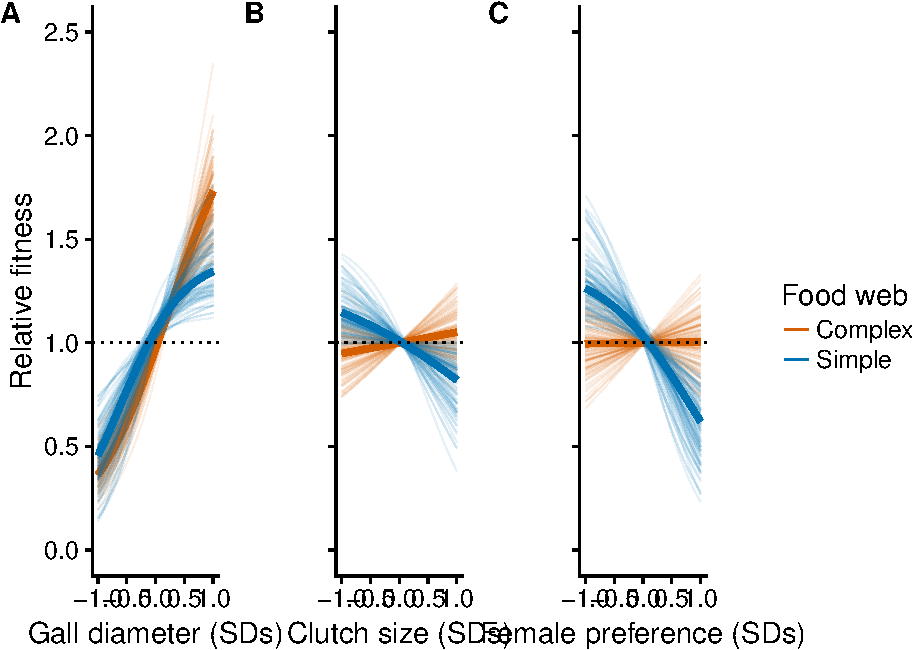
\includegraphics{elsevier_test_files/figure-latex/Plot Univariate Landscapes-1.pdf}

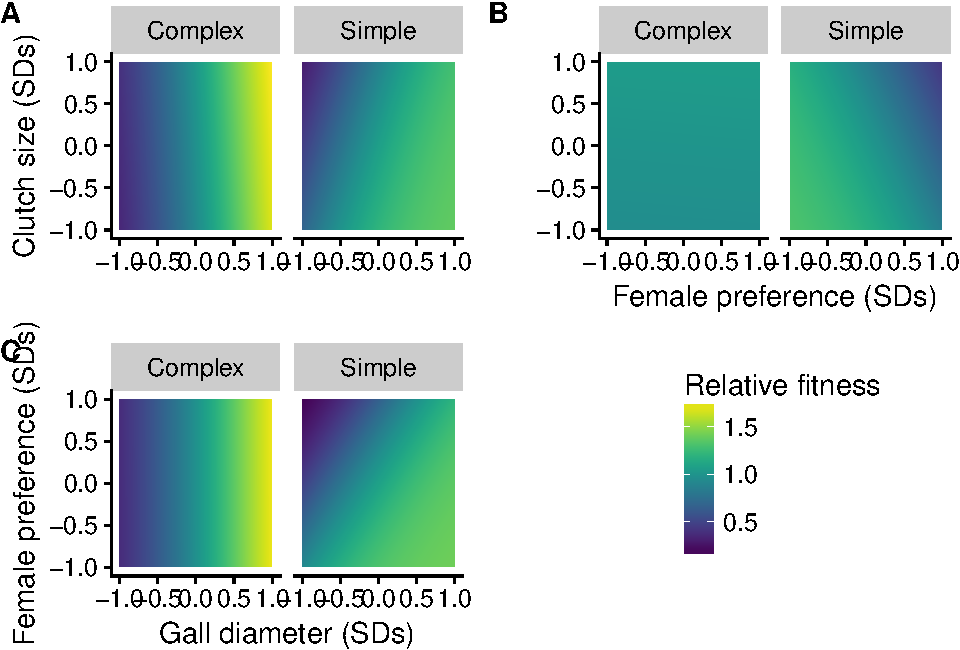
\includegraphics{elsevier_test_files/figure-latex/Plot Multivariate Fitness Landscape-1.pdf}

\begin{verbatim}
##              df      AIC
## beta_control  7 809.1027
## quad_control 10 814.3022
## corr_control 13 817.6910
\end{verbatim}

\begin{verbatim}
##                  df      AIC
## beta_control      7 809.1027
## glm.beta_control  4 881.0152
\end{verbatim}

\begin{verbatim}
##                           df      AIC
## beta_control               7 809.1027
## beta_control.REonlyGallID  5 816.4817
\end{verbatim}

\begin{verbatim}
##       chisq       ratio         rdf           p 
## 349.7811634   0.5025591 696.0000000   1.0000000
\end{verbatim}

\begin{verbatim}
##                df      AIC
## beta_treatment  7 619.1030
## quad_treatment 10 620.1640
## corr_treatment 13 622.3247
\end{verbatim}

\begin{verbatim}
##       chisq       ratio         rdf           p 
## 190.3351784   0.3215121 592.0000000   1.0000000
\end{verbatim}

\begin{verbatim}
##                    df      AIC
## beta_treatment      7 619.1030
## glm.beta_treatment  4 712.4146
\end{verbatim}

\begin{verbatim}
##                             df      AIC
## beta_treatment               7 619.1030
## beta_treatment.REonlyGallID  6 669.5617
\end{verbatim}

\begin{verbatim}
## Data: treatment_df
## Models:
## beta_treatment.REonlyGallID: gall_survival ~ sc.gall_size + sc.clutch_size + sc.female_preference + 
## beta_treatment.REonlyGallID:     (1 | Genotype/Plant_Position)
## beta_treatment: gall_survival ~ sc.gall_size + sc.clutch_size + sc.female_preference + 
## beta_treatment:     (1 | Genotype/Plant_Position/Gall_Number)
##                             Df    AIC    BIC  logLik deviance  Chisq
## beta_treatment.REonlyGallID  6 669.56 695.93 -328.78   657.56       
## beta_treatment               7 619.10 649.87 -302.55   605.10 52.459
##                             Chi Df Pr(>Chisq)    
## beta_treatment.REonlyGallID                      
## beta_treatment                   1  4.394e-13 ***
## ---
## Signif. codes:  0 '***' 0.001 '**' 0.01 '*' 0.05 '.' 0.1 ' ' 1
\end{verbatim}

\begin{verbatim}
## Data: treatment_df
## Models:
## glm.beta_treatment: gall_survival ~ sc.gall_size + sc.clutch_size + sc.female_preference
## beta_treatment: gall_survival ~ sc.gall_size + sc.clutch_size + sc.female_preference + 
## beta_treatment:     (1 | Genotype/Plant_Position/Gall_Number)
##                    Df    AIC    BIC  logLik deviance  Chisq Chi Df
## glm.beta_treatment  4 712.41 730.00 -352.21   704.41              
## beta_treatment      7 619.10 649.87 -302.55   605.10 99.311      3
##                    Pr(>Chisq)    
## glm.beta_treatment               
## beta_treatment      < 2.2e-16 ***
## ---
## Signif. codes:  0 '***' 0.001 '**' 0.01 '*' 0.05 '.' 0.1 ' ' 1
\end{verbatim}

\section{Discussion}\label{discussion}

More recently, researchers have begun to explore how the community
context drives evolutionary change (Mcpeek (2017); terHorst et al.
(2018)).

NEED to recognize that evolutionary biologists have begun to explore how
community context affects evolutionary change (work by Sharon Strauss,
Casey terHorst, Lutz Becks, etc.). These results have begun to show
interesting patterns whereby the composition of species in a community
can alter the direction and strength of natural selection imposed on
species embedded within these communities (cite).

In other words, these results have begun to illustrate show how
biological diversity, in terms of differences between species, can shape
evolution. Nevertheless, predicting the how the composition of species
in a community requires moving beyond a description of community
composition. simply knowing the composition of species in a community
will

There are various bibliography styles available. You can select the
style of your choice in the preamble of this document. These styles are
Elsevier styles based on standard styles like Harvard and Vancouver.
Please use BibTeX~to generate your bibliography and include DOIs
whenever available.

Here are two sample references: ({\textbf{???}}; {\textbf{???}}).

\section*{References}\label{references}
\addcontentsline{toc}{section}{References}

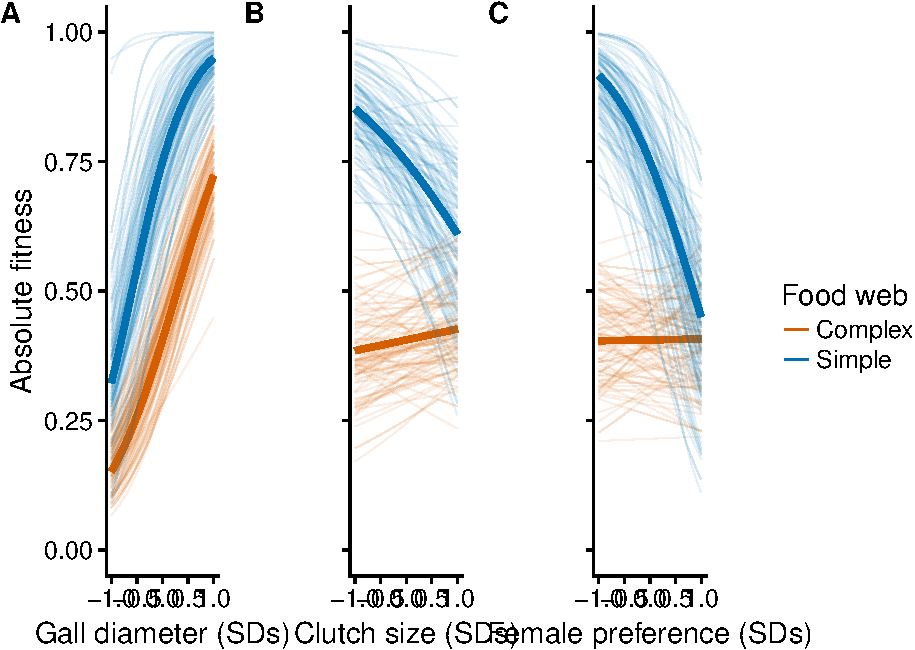
\includegraphics{elsevier_test_files/figure-latex/Univariate Absolute Fitness Landscapes-1.pdf}

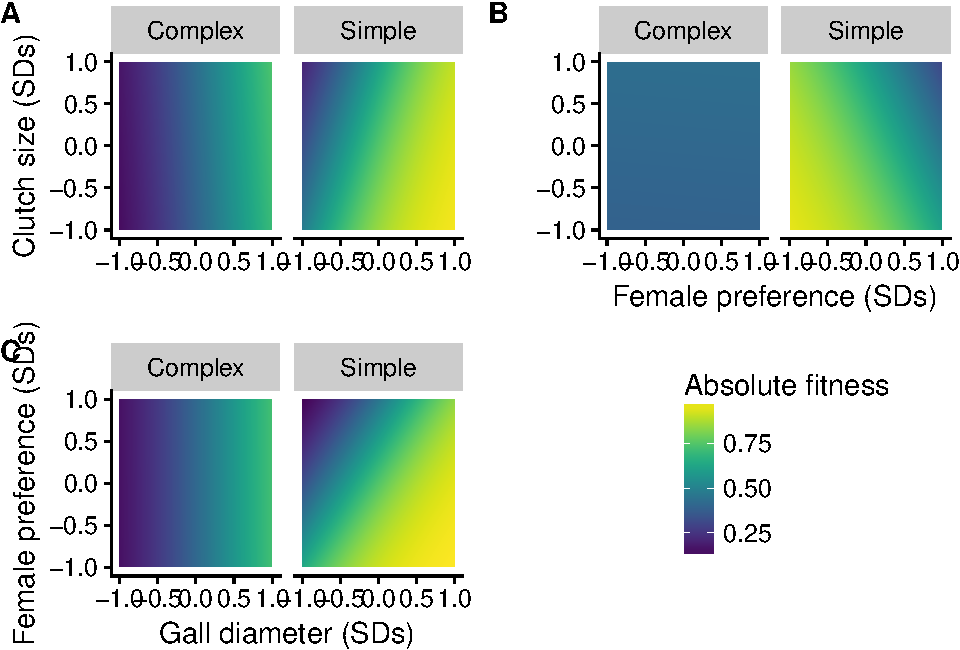
\includegraphics{elsevier_test_files/figure-latex/Multivariate Absolute Fitness Landscapes-1.pdf}

\hypertarget{refs}{}
\hypertarget{ref-Abrams2000}{}
Abrams, Peter A. 2000. ``The Evolution of Predator-Prey Interactions:
Theory and Evidence.'' \emph{Annu. Rev. Ecol. Syst.} 31. Annual Reviews:
79--105.

\hypertarget{ref-Banasek-Richter2009}{}
Banasek-Richter, Carolin, Louis-Félix Bersier, Marie-France Cattin,
Richard Baltensperger, Jean-Pierre Gabriel, Yves Merz, Robert E
Ulanowicz, et al. 2009. ``Complexity in Quantitative Food Webs.''
\emph{Ecology} 90 (6): 1470--7.

\hypertarget{ref-Barbour2016}{}
Barbour, Matthew A, Miguel A Fortuna, Jordi Bascompte, Joshua R
Nicholson, Riitta Julkunen-Tiitto, Erik S Jules, and Gregory M
Crutsinger. 2016. ``Genetic Specificity of a Plant--insect Food Web:
Implications for Linking Genetic Variation to Network Complexity.''
\emph{Proceedings of the National Academy of Sciences} 113 (8). National
Acad Sciences: 2128--33.

\hypertarget{ref-Barbour2015}{}
Barbour, Matthew A, Mariano A Rodriguez-Cabal, Elizabeth T Wu, Riitta
Julkunen-Tiitto, Carol E Ritland, Allyson E Miscampbell, Erik S Jules,
and Gregory M Crutsinger. 2015. ``Multiple Plant Traits Shape the
Genetic Basis of Herbivore Community Assembly.'' \emph{Funct. Ecol.} 29
(8): 995--1006.

\hypertarget{ref-Bolker2009}{}
Bolker, Benjamin M, Mollie E Brooks, Connie J Clark, Shane W Geange,
John R Poulsen, M Henry H Stevens, and Jada-Simone S White. 2009.
``Generalized Linear Mixed Models: A Practical Guide for Ecology and
Evolution.'' \emph{Trends Ecol. Evol.} 24 (3): 127--35.

\hypertarget{ref-Janzen1998}{}
Frederic J Janzen and Hal S Stearn. 1998. ``Logistic Regression for
Empirical Studies of Multivariate Selection.'' \emph{Evolution} 52 (6):
1564--71.

\hypertarget{ref-Gripenberg2010}{}
Gripenberg, Sofia, Peter J Mayhew, Mark Parnell, and Tomas Roslin. 2010.
``A Meta-Analysis of Preference-Performance Relationships in
Phytophagous Insects.'' \emph{Ecol. Lett.} 13 (3): 383--93.

\hypertarget{ref-Guimaraes2017}{}
Guimarães, Paulo R, Jr, Mathias M Pires, Pedro Jordano, Jordi Bascompte,
and John N Thompson. 2017. ``Indirect Effects Drive Coevolution in
Mutualistic Networks.'' \emph{Nature} 550 (7677): 511--14.

\hypertarget{ref-Hawkins1997}{}
Hawkins, Bradford A, Howard V Cornell, and Michael E Hochberg. 1997.
``Predators, Parasitoids, and Pathogens as Mortality Agents in
Phytophagous Insect Populations.'' \emph{Ecology} 78 (7). Ecological
Society of America: 2145--52.

\hypertarget{ref-Heath2018}{}
Heath, Jeremy J, Patrick Abbot, and John O Stireman 3rd. 2018.
``Adaptive Divergence in a Defense Symbiosis Driven from the Top down.''
\emph{Am. Nat.} 192 (1): E21--E36.

\hypertarget{ref-Hunter2018}{}
Hunter, Darren C, Josephine M Pemberton, Jill G Pilkington, and Michael
B Morrissey. 2018. ``Quantification and Decomposition of
Environment-Selection Relationships.'' \emph{Evolution}, March.

\hypertarget{ref-Ives2005}{}
Ives, Anthony R, Bradley J Cardinale, and William E Snyder. 2005. ``A
Synthesis of Subdisciplines: Predator--prey Interactions, and
Biodiversity and Ecosystem Functioning.'' \emph{Ecol. Lett.} 8 (1).
Blackwell Science Ltd: 102--16.

\hypertarget{ref-Janzen1974}{}
Janzen, Daniel. 1974. ``The Deflowering of Central America.''
\emph{Natural History} 83 (January): 49--53.

\hypertarget{ref-Jordano1987}{}
Jordano, Pedro. 1987. ``Patterns of Mutualistic Interactions in
Pollination and Seed Dispersal: Connectance, Dependence Asymmetries, and
Coevolution.'' \emph{Am. Nat.} 129 (5): 657--77.

\hypertarget{ref-De_Mazancourt2008}{}
Mazancourt, C de, E Johnson, and T G Barraclough. 2008. ``Biodiversity
Inhibits Species' Evolutionary Responses to Changing Environments.''
\emph{Ecol. Lett.} 11 (4): 380--88.

\hypertarget{ref-McPeek2017}{}
Mcpeek, Mark A. 2017. \emph{Evolutionary Community Ecology}. Princeton
University Press.

\hypertarget{ref-Nuismer2013}{}
Nuismer, Scott L, Pedro Jordano, and Jordi Bascompte. 2013.
``Coevolution and the Architecture of Mutualistic Networks.''
\emph{Evolution} 67 (2): 338--54.

\hypertarget{ref-R2018}{}
R Core Team. 2018. \emph{R: A Language and Environment for Statistical
Computing}. Vienna, Austria: R Foundation for Statistical Computing.
\url{https://www.R-project.org/}.

\hypertarget{ref-Russo2006}{}
Russo, Ron. 2006. \emph{Field Guide to Plant Galls of California and
Other Western States}. 1st ed. University of California Press.

\hypertarget{ref-Schluter2000}{}
Schluter, Dolph. 2000. ``Ecological Character Displacement in Adaptive
Radiation.'' \emph{Am. Nat.} 156 (S4): S4--S16.

\hypertarget{ref-Singer1986}{}
Singer, Michael C. 1986. ``The Definition and Measurement of Oviposition
Preference in Plant-Feeding Insects.'' In \emph{Insect-Plant
Interactions}, edited by James R Miller and Thomas A Miller, 65--94. New
York, NY: Springer New York.

\hypertarget{ref-TerHorst2018}{}
terHorst, Casey P, Peter C Zee, Katy D Heath, Thomas E Miller, Abigail I
Pastore, Swati Patel, Sebastian J Schreiber, Michael J Wade, and Matthew
R Walsh. 2018. ``Evolution in a Community Context: Trait Responses to
Multiple Species Interactions*.'' \emph{Am. Nat.}, January. University
of Chicago PressChicago, IL.

\hypertarget{ref-Weis1983}{}
Weis, Arthur E, Peter W Price, and Michael Lynch. 1983. ``Selective
Pressures on Clutch Size in the Gall Maker Asteromyia Carbonifera.''
\emph{Ecology} 64 (4). Ecological Society of America: 688--95.

\end{document}


